
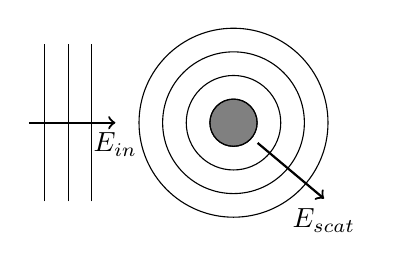
\begin{tikzpicture}%[every node/.style={draw,outer sep=0pt,thick}]


\draw[fill=gray] (0,0) circle (3mm);

\foreach \u in {1,2,3,4}{
	\draw[] (0,0) circle (\u * 3mm);
}

\foreach \u in {2,3,4}{
	\draw[] (-30mm + \u * 3mm,-1) --  ++ (0,2);
}

\draw[->, thick] (-26mm,0) -- (-15mm,0) node [below] {$E_{in}$};
\draw[->, thick] (-0,0)  + (-40:4mm) -- ++ (-40:15mm) node [below] {$E_{scat}$};

%
%\foreach \u in {1,2,3}{
%	\draw[] (6mm + \u * 3mm,-1) --  ++ (0,2);
%}
%
%\draw[->, thick] (4mm,4mm) -- ++ (11mm,0) node [right] {$E_{in}$};
%\draw[->, thick] (4mm,0)  -- ++ (0:11mm) node [right] {$E_{scat}$};
%


\end{tikzpicture}

